\documentclass[hyperref={pdfpagelabels=false}]{beamer}
\usepackage{lmodern,amsmath,physics,subcaption}

\def\signed #1{{\leavevmode\unskip\nobreak\hfil\penalty50\hskip1em
  \hbox{}\nobreak\hfill #1%
  \parfillskip=0pt \finalhyphendemerits=0 \endgraf}}

\newsavebox\mybox
\newenvironment{aquote}[1]
  {\savebox\mybox{#1}\begin{quote}\openautoquote\hspace*{-.7ex}}
  {\unskip\closeautoquote\vspace*{1mm}\signed{\usebox\mybox}\end{quote}}
  
%\definecolor{UV}{rgb}{0.58, 0.0, 0.83}
\usetheme{Marburg}
\setbeamertemplate{sidebar canvas right}[vertical shading][top=black,bottom=blue]
\usecolortheme{sidebartab}
\usecolortheme[named=blue]{structure}
\usefonttheme{serif}
\title{Title}
\author{Martin Sjöborg} 
%\date{\today} 
\begin{document}
\begin{frame}
\titlepage
\end{frame} 


\begin{frame}
\frametitle{Contents}
\tableofcontents[pausesubsections]
\end{frame} 


\section{Section 1} 
\subsection{Subsection 1}
\begin{frame}
\frametitle{Subsection 1} 
\begin{align}
    \mathcal{G}_X \times \mathcal{G}_{SM} \to \mathcal{G}_{SM} \nonumber 
\end{align}
\end{frame}

\section{Section 2} 
\subsection{Subsection 2}
\begin{frame}
\frametitle{Subsection 2} 
\begin{figure}
    \centering
    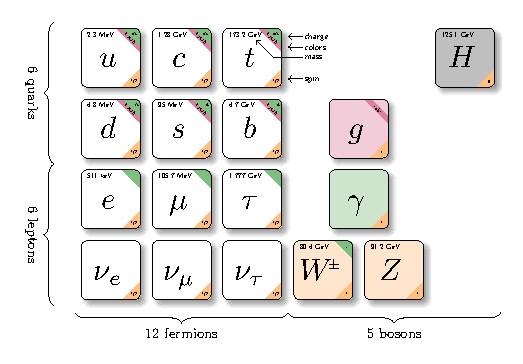
\includegraphics[scale = 1]{SM_1.pdf}
\end{figure}
\end{frame}
\end{document}
